\subsection{Capacity Evaluation}
\label{sec-eval-capacity}
\begin{figure}[t]
    \begin{subfigure}[b]{0.5\textwidth}
        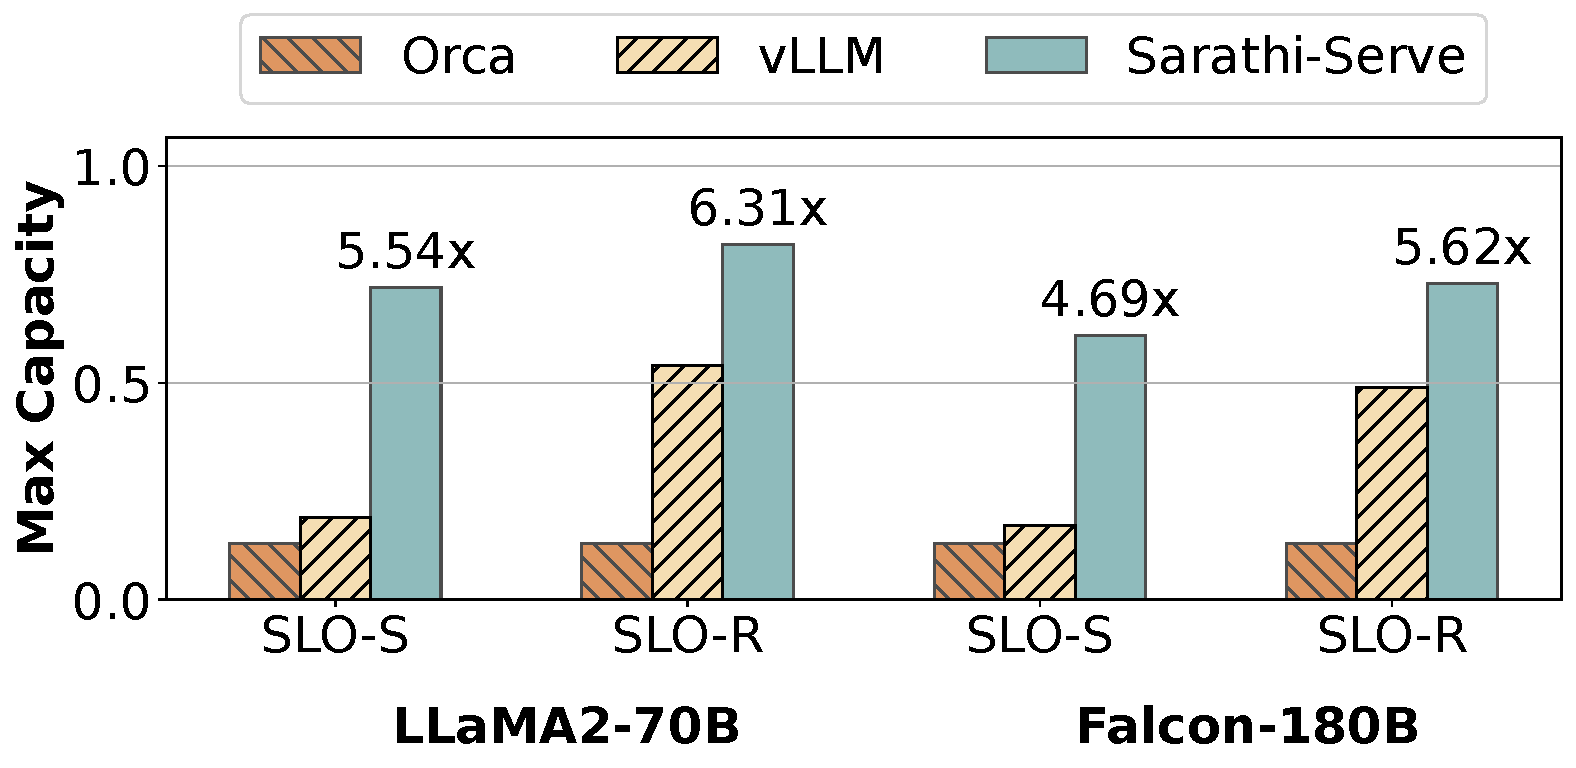
\includegraphics[width=0.95\textwidth]{figures/capacity-plots-pp-openchat.pdf}
        \caption{Dataset: \sharegpt.}
        \label{fig:eval:capacity:pp:openchat}
    \end{subfigure}
    \\
    \begin{subfigure}[b]{0.5\textwidth}
        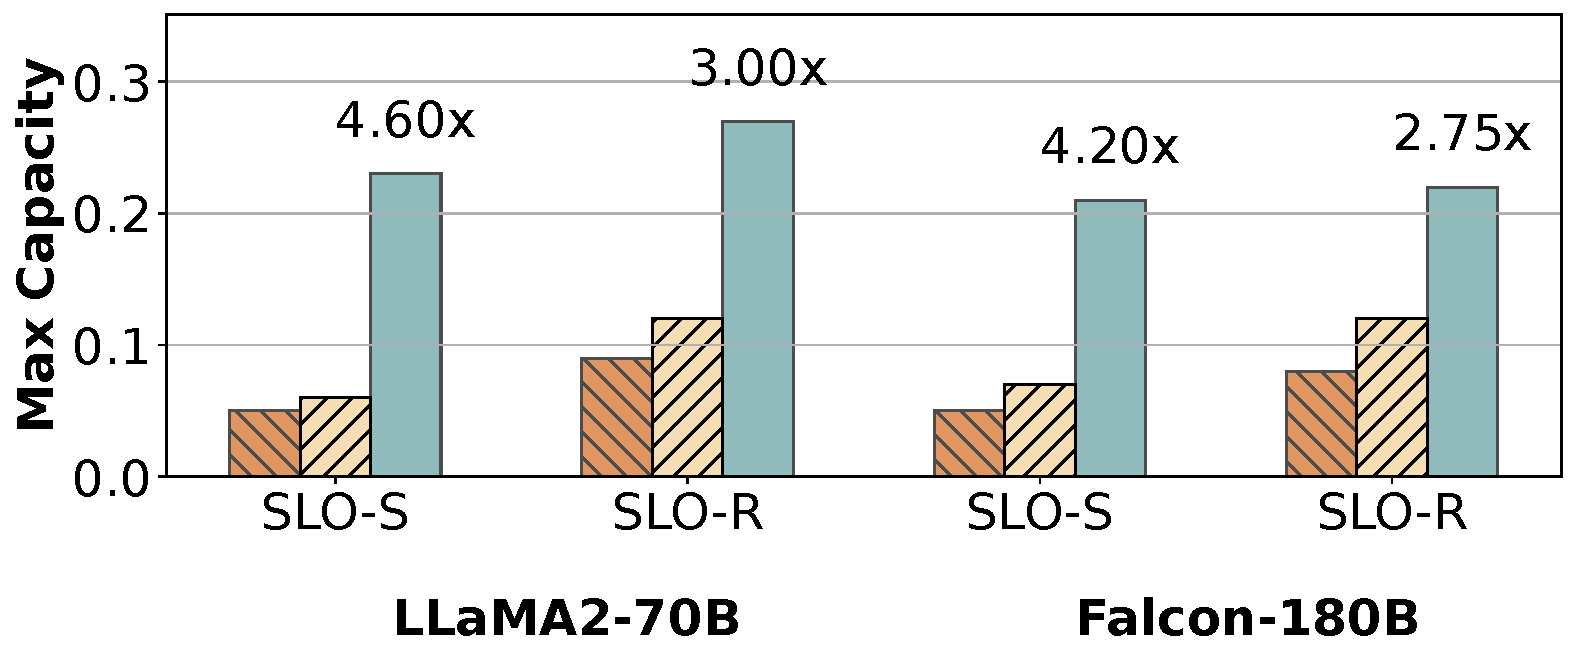
\includegraphics[width=0.95\textwidth]{figures/capacity-plots-pp-arxiv.pdf}
        \caption{Dataset: \arxivsum.}
        \label{fig:eval:capacity:pp:arxiv}
    \end{subfigure}
    \caption{Capacity of \llamaL and \falcon (models with pipeline parallelism) with different schedulers under strict (SLO-S) and relaxed (SLO-R) latency SLOs.}
    \label{fig:eval:capacitypp}
\end{figure}

We evaluate \sysname, Orca and vLLM on all four models and both datasets under two different latency configurations: \relaxed and \strict. Similar to Patel et al. \cite{patel2023splitwise}, to account for the intrinsic performance limitations of a model and hardware pair, we define the \slo on P99 TBT to be equal to 5\myx and 25\myx the execution time of a decode iteration for a request (with prefill length of 4k and 32 batch size) running without any prefill interference for the \strict and \relaxed settings, respectively. %
~\autoref{table:eval:slos} shows a summary of the absolute \slo thresholds. Note that the \strict SLO represents the latency target desired for interactive applications like chatbots. On the other hand, the \relaxed configuration is exemplary of systems where the complete sequence of output tokens should be generated within a predictable time limit but the TBT constraints on individual tokens is not very strict. For all load experiments, we ensure that the maximum load is sustainable, i.e., the queuing delay does not blow up (we use a limit of 2 seconds on median scheduling delay).


\autoref{fig:eval:capacitytp} and~\autoref{fig:eval:capacitypp} show the results of our capacity experiments. \sysname consistently outperforms Orca and vLLM in all cases across models and workloads. Under \strict \slo, \sysname can sustain up to $4.0\times$ higher load compared to Orca and $3.7\times$ higher load than vLLM under \strict \slo (\yi, \sharegpt). For larger models using pipeline parallelism, \sysname achieves gains of up to 6.3\myx and 4.3\myx compared to Orca and vLLM respectively (\llamaL, \sharegpt) due to few pipeline bubbles.


We observe that in most scenarios, Orca and vLLM violate the P99 TBT latency \slo before they can reach their maximum serviceable throughput. Thus, we observe relaxing the latency target leads to considerable increase in their model serving capacity. In \sysname, one can adjust the chunk size based on the desired SLO. Therefore, we use a strict token budget and split prompts into smaller chunks when operating under \strict latency \slo. This reduces system efficiency marginally but allows us to achieve lower tail latency. On the other hand, when the latency constraint is relaxed, we increase the token budget to allow more efficient prefills. We use token budget of 2048 and 512 for all models under the \relaxed and \strict settings,  respectively, except for the \llamaL \relaxed configuration where we use token budget of 1536 to reduce the impact of pipeline bubbles. The system performance can be further enhanced by dynamically varying the token budget based on workload characteristics. We leave this exploration for future work.


We further notice that vLLM significantly outperforms Orca under relaxed setting. The reason for this is two-fold. First, Orca batches prompts for multiple requests together ({\it max sequence length * batch size} compared to {\it max sequence length} in vLLM), which can lead to even higher tail latency in some cases. Second, vLLM supports a much larger batch size compared to Orca. The lower batch size in Orca is due to the lack of PagedAttention and the large activation memory footprint associated with processing batches with excessively large number of tokens.

Finally, note that the capacity of each system is higher for \sharegpt dataset compared to the \arxivsum dataset. This is expected because prompts in the \arxivsum datasets are much longer - 7059 vs 1730 median tokens as shown in~\autoref{table:eval:datasets}. The larger prompts makes Orca and vLLM more susceptible to latency violations due to higher processing time of these longer prefills.%



 \subsection{Throughput-Latency Tradeoff}
\label{subsec-tput-latency}

To fully understand the throughput-latency tradeoff in LLM serving systems, we vary the P99 TBT latency SLO and observe the impact on system capacity for vLLM and \sysname. ~\autoref{fig:eval:lateny-tput-tradeoff} shows the results for \mistral and \yi models with five different SLO values for the \sharegpt dataset.

We evaluate vLLM with three different batch sizes in an attempt to navigate the latency-throughput trade-off as prescribed by Yu et al. \cite{orca}. The maximum capacity of vLLM gets capped due to generation stalls under stringent TBT SLOs. Notably, the capacity of vLLM remains largely identical for all the three batch size settings. This implies that even though PagedAttention enables large batch sizes with efficient memory management -- in practical situations with latency constraints, vLLM cannot leverage the large batch size due to the steep latency-throughput tradeoff made by it's \prefillprio scheduler.

On the other hand, the latency-throughput tradeoff in \sysname can be precisely controlled by varying the token budget. \sysname achieves 3.5\myx higher capacity compared to vLLM under strict SLO (100ms, \mistral) using a small token budget of 512. For scenarios with more relaxed SLO constraints, picking a larger token budget of 2048 allows \sysname to operate more efficiently resulting in 1.65\myx higher capacity compared to vLLM (1s, \yi).







\begin{figure}[t!]
\centering
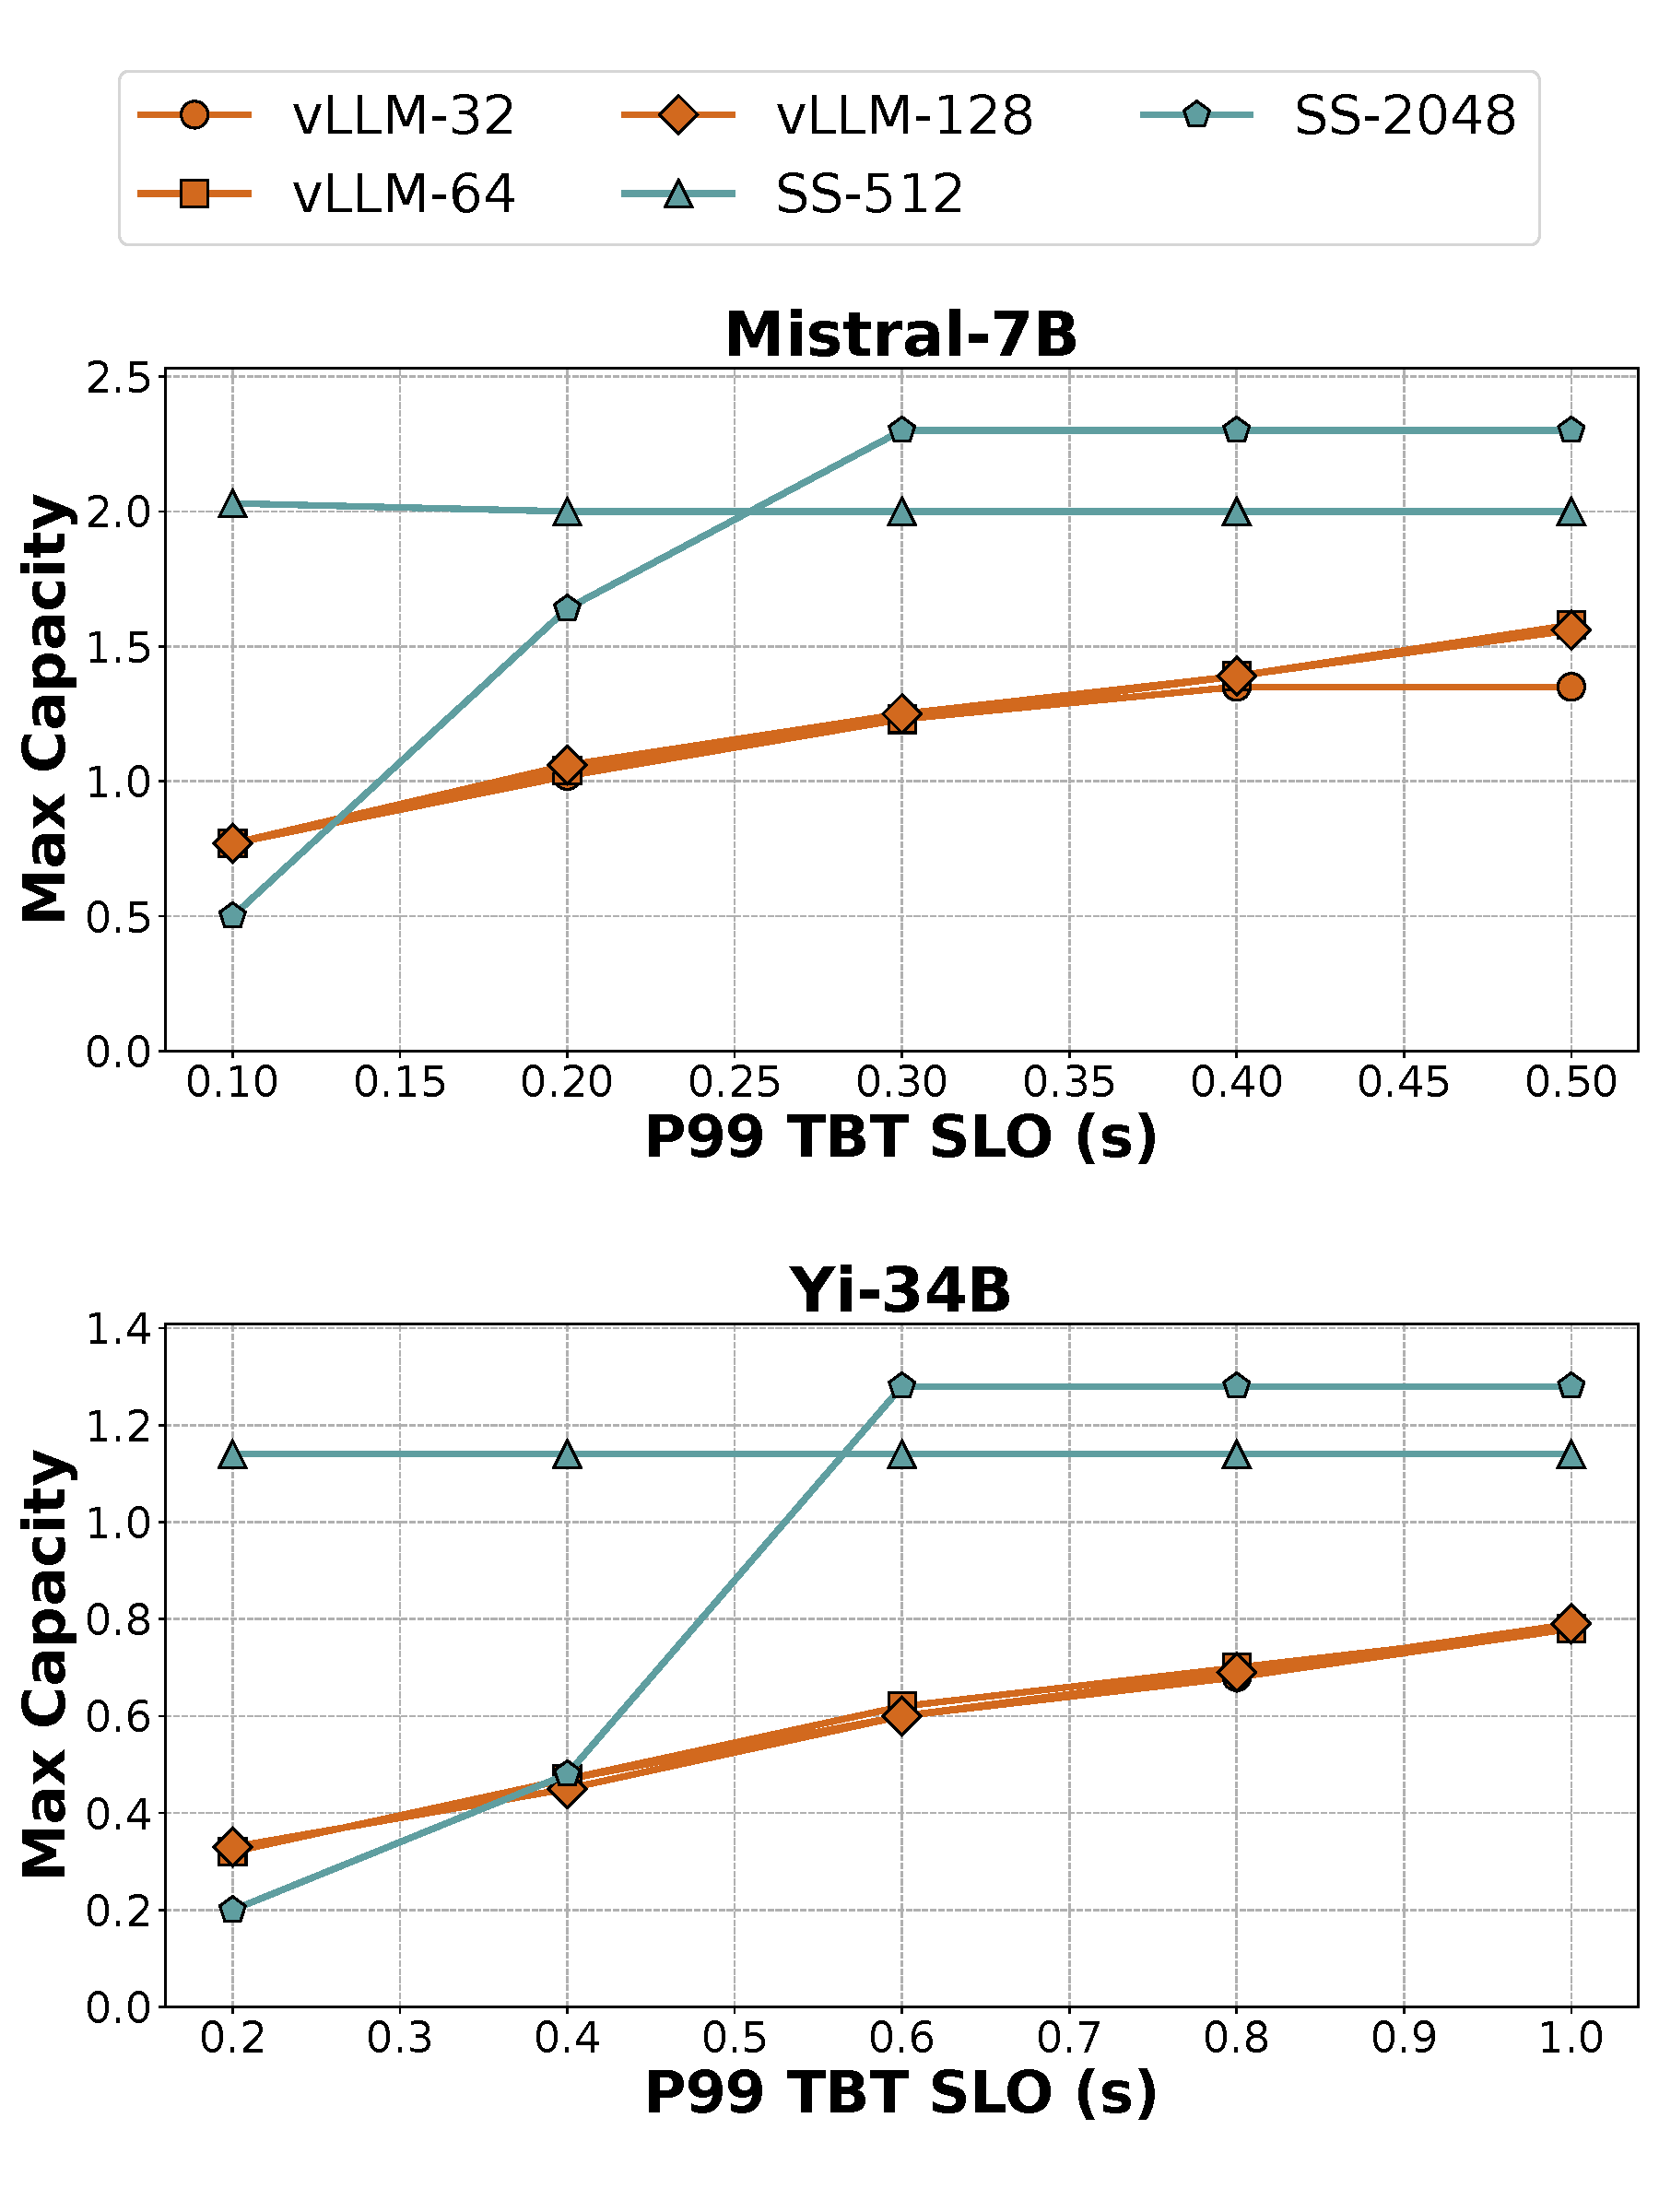
\includegraphics[width=0.95\linewidth]{figures/latency_tradeoff.pdf}
    \caption{Latency -- Throughput tradeoff in vLLM and \sysname for \mistral and \yi models on \sharegpt dataset. We evaluate vLLM with three different max batch sizes of 32, 64 and 128. For \sysname, we consider token budget of 512 and 2048 with max batch size of 128.
    \sysname delivers 3.5\myx higher capacity under stringent SLOs for \yi using \Hbatch.}
    \label{fig:eval:lateny-tput-tradeoff}
\end{figure}

